\section{Meta learning for Erd\"{o}s Goes Neural (\proj)}
%\subsection{\proj}
The above performance guarantee lays the theoretical foundation for EGN. However, the following practical issue motivates us to incorporate meta learning into EGN.
%the unsupervised learning framework.

\subsection{Motivation: What needed is learning for instance-wise good solutions}
 It is often time-consuming to perform online optimization of $l(\theta;G)$ for each encountered instance $G$. This also mismatches the goal of learning, i.e., learning heuristics from history/data. Therefore, a  pipeline commonly adopted is as follows. Suppose there is a set of training instances $G_i$, $1\leq i\leq m$, IID sampled from a distribution $\mathbb{P}_{\mathcal{G}}$. We optimize $\theta$ by following 
\begin{equation}
\label{eq:previous_goal}
\begin{aligned}
\min_{\theta} \;\sum_{i=1}^m l(\theta;G_i),
\end{aligned}
\end{equation}
which is similar to empirical risk minimization (ERM) in standard supervised learning. When a test instance $G$ appears, we apply the learned $\mathcal{A}_{\theta}$ to get a soft solution and round it to the final solution.

This pipeline cannot guarantee the quality for this instance $G$. Even if the training instances $G_i$, $1\leq i\leq m$ are in a large quantity (so in-distribution generalization is not a problem), and even if the test instance $G$ also follows $\mathbb{P}_{\mathcal{G}}$, we may not guarantee a low $l(\theta;G)$ for one particular $G$ because ERM only guarantees a low averaged performance $\mathbb{E}_{G\sim\mathbb{P}_{\mathcal{G}}}[l(\theta;G)]$.  This issue may also violate the condition to have a performance guarantee as reviewed in Sec.~\ref{sec:prelim}, as it is instance-wise. Here, we highlight that in practice even the minimal averaged loss $\min_{\theta} \mathbb{E}_{G\sim\mathbb{P}_{\mathcal{G}}}[l(\theta;G)]$ is often strictly greater than averaged instance-wise minimal loss $\mathbb{E}_{G\sim\mathbb{P}_{\mathcal{G}}}[\min_{\theta} l(\theta;G)]$, because practical NNs are not expressive enough to remember the optimal solution to every instance.% due to the complex structure of a CO problem~\citep{}.     %may not be further applied. 

Unfortunately, many practical CO problems actually expect \emph{instance-wise good solutions}. This is because every instance in practice is crucial. A terrible solution for one instance may raise a security issue (e.g., the surveillance-camera allocation problem) or cause huge economic losses (e.g., the routing problem in a transportation system). With this observation, our work is to address the problem by studying \emph{unsupervised learning for instance-wise good solutions to CO problems}.

%: For each encountered test instance $G$, a solution $X$ of good quality is needed.

%Practical CO problems often expect \emph{instance-wise good solutions}: For each encountered test instance $G$, a solution $X$ of good quality is needed. This is because every instance in practice is crucial. A terrible solution for one instance may raise security issue (e.g., the surveillance-camera allocation problem) or cause huge economic losses (e.g., the routing problem in a transportation system). However,

%\pan{The following is something used before}

% In theory, by minimizing Eq.~\ref{eq:previous_goal}, if a test instance $G$ follows $\mathbb{P}_{\mathcal{G}}$, directly apply the learned $\mathcal{A}_{\theta}$ to $G$ may expect to have a low $l(\theta;G)$

% an empirical risk minimization (ERM)        

% \cite{karalias2020erdos,wang2022unsupervised}

% IID sampled from a distribution $\mathbb{P}_{\mathcal{G}}$

% Suppose the training instances $G_i$, $1\leq i\leq m$ are IID sampled from a distribution $\mathbb{P}_{\mathcal{G}}$,  \cite{karalias2020erdos,wang2022unsupervised} optimize $\theta$ by following an empirical risk minimization (ERM)
% \begin{equation}
% \label{eq:previous_goal}
% \begin{aligned}
% \min_{\theta} \;\sum_{i=1}^m l(\theta;G_i).
% \end{aligned}
% \end{equation}
% This framework expects that by optimizing Eq.~\ref{eq:previous_goal}, the NN $\mathcal{A}_{\theta}$ can learn heuristics to generate a soft solution $\bar{X}=\mathcal{A}_{\theta}(G)$ for graph instances $G\sim\mathbb{P}_{\mathcal{G}}$. 


% %Therefore, if the test instances $G_i$, 
% %$m+1\leq i\leq m+q$ follow the same d  


% One expects the NN to learn heuristics by training $\theta$ over $\Xi$. 

% Suppose the set of training instances $\Xi=\{G_1,G_2,...,G_m\}$,
% By assuming a distribution of graph instances $\mathbb{P}_{\mathcal{G}}$
% assumes that there is a distribution of graph instances $\mathbb{P}_$


% The framework asks to relax the original objective: The relaxed cost function $f_r(\cdot;G):[0,1]^n \rightarrow \mathbb{R}_{\geq0}$ where $f_r(X;G)=f(X;G)$ on any discrete points $$ 

% learn a parameterized algorithm $\mathcal{A}_{\theta}(\cdot):\mathcal{G}\rightarrow \{0,1\}^n$, which give
 
% %Here, we use the notation in~\cite{wang2022unsupervised}. EGN   The unsupervised learning for CO framework~\cite{wang2022unsupervised}

% The unsupervised learning for CO framework~\cite{wang2022unsupervised} could be summarized as training a parameterized algorithm $\mathcal{A}_{\theta}$ with the loss function below:
% \begin{equation}
% \label{method:previous_loss}
% \begin{aligned}
% l(\theta;G) \triangleq f(\bar{X};G) + \beta g(\bar{X};G) , \quad \bar{X} = \mathcal{A}_{\theta}(G)
% \end{aligned}
% \end{equation}, where $f$ is the cost function and $g$ represents the penalty constraints such that $\Omega \triangleq \{X\in\{0,1\}^n: g(X;G) = 0\}, \stcomp{\Omega} \triangleq \{X\in\{0,1\}^n: g(X;G) \geq 1\}$. $\theta$ denotes the parameters of the neural network,  $\bar{X} \in [0,1]^n$ denotes the vector embeddings relaxed to continuous space, $\beta > \max_{X\in \Omega} f(X;G)$ is the penalty coefficient hyper-parameter. Note that the probabilistic loss function of EGN~\citep{karalias2020erdos} could also be adapted into the same form as above. The optimization goal of the unsupervised learning framework, is to minimize the population-level loss function in the expectation sense over a certain data distribution $G \sim \mathbb{P}_G$ in space $\mathcal{G}$:
% \begin{equation}
% \label{method:previous_goal}
% \begin{aligned}
% \min_{\theta} \mathbb{E}_{G\sim \mathbb{P}_G} l(\theta;G).
% \end{aligned}
% \end{equation}
% When encountered a testing instance $G'$, once the loss value achieves $l(\theta;G')<\beta$, a feasible solution $X=R(\mathcal{A}_{\theta}(G'))$ with performance guarantee $f(X;G') \leq l(\theta;G')$ could be generated via the rounding process $R(\cdot)$ as shown in Def.~\ref{method:def_rounding} below.
% \begin{definition}[Rounding]
% \vspace{-0.3cm}
% \label{method:def_rounding}
% For a continuous embedding $\bar{X} \in [0,1]^n$ and an arbitrary order of the entries (w.l.o.g 1,2,...,n), fix all the other entries unchanged and round $\bar{X}_i$ into $0$ or $1$ as $X_i = \arg\min_{j=0,1} f(X_1,...,X_{i-1},j,\bar{X}_{i+1},...,\bar{X}_n)+\beta g(X_1,...,X_{i-1},j,\bar{X}_{i+1},...,\bar{X}_n)$, replace $\bar{X}_i$ with $X_i$ and repeat this operation until all the entries are discrete.
% \vspace{-0.2cm}
% \end{definition}

%\subsection{}
% However, even if the obtained algorithm $\mathcal{A}_{\theta}$ manages to minimize the objective $\min_{\theta} \mathbb{E}_{G\sim \mathbb{P}_G} l(\theta;G)$, there is still no guarantee that the rounded solution $X=R(\mathcal{A}_{\theta}(G))$ would achieve optimality for the actual objective of CO $\min_{X} f(X;G)$ given any unseen $G \in \mathcal{G}$, with $R(\cdot)$ denoting the rounding procedure. Because there always \pan{always sounds a little bit overemphasis. You just need to say they are different.} exists a gap between the optimality in the expectation sense in Eq.~\ref{method:previous_goal} and the optimality for a single instance in Eq.~\ref{method:def_CO}. Let $Tr(\mathbb{P}_G)$ \pan{Bad notation} denote the training dataset sampled from $\mathbb{P}_G$, only if neural networks could not only remember the optimal solution $\arg\min_{X}f(X;G)$ of every training instance $G \in Tr(\mathbb{P}_G)$ to its optimal solution $\arg\min_{X}f(X;G)$, but also perform totally correct generalization on any unseen data $G' \in \mathcal{G} \backslash Tr(\mathbb{P}_G)$, shall the gap be erased. This is practically unrealistic due to the limitation on the models' expressive power\hl{reference} and the dataset volume~\citep{yehuda2020s}. Thus in practice, the cost obtained by optimizing the objective over expectation should be always greater or equal to the optimal solution for a single instance:  
% \begin{equation}
% \label{method:eq_gap}
% \begin{aligned}
% \forall G \in \mathcal{G}, \quad f(R(\mathcal{A}_{\theta}(G));G) \geq f(\arg\min_X f(X;G);G)
% \end{aligned}
% \end{equation}

\subsection{Training towards instance-wise optimality via Meta Learning}

Our idea to address the problem is to regard the goal of learning from history as to search for good initialization for future instances rather than give direct solutions. Such good initialization can be quickly fine-tuned by further optimizing the model for each instance, which ultimately gives instance-wise good solutions. However, in practice, we do not have access to any future/test instances. So, can we just use historical/training instances to implement the above idea? Our strategy is to view each training instance $G_i$ as a pseudo-test instance to test and optimize the quality of initialization given by the model. Specifically, this strategy gives us an objective
\begin{equation}
\label{eq:infinite_step}
\begin{aligned}
\min_{\theta} \;\sum_{i=1}^m \tilde{l}_i(\theta), \quad \text{where}\; \tilde{l}_i(\theta) = \min_{\theta_i} l(\theta_i;G_i) \;\text{with $\theta_i=\theta$ as initialization.}
\end{aligned}
\end{equation}
Eq.~\ref{eq:infinite_step} has some abuse of notations. The minimum $\tilde{l}_i(\theta)$  depending on the initialization $\theta$ is because of the non-convex nature of  $\min_{\theta_i} l(\theta_i;G_i)$, where the initialization $\theta_i=\theta$ matters significantly. 

\begin{algorithm}[t]
\caption{Train \proj and Test \proj with/without Fine-tuning}
\label{method:alg_table}
\begin{algorithmic}[1]
\Require Training instances $\Xi=\{G_1,G_2,...,G_m\}$; Hyperparameters: $\alpha, \gamma$.
\State Randomly initialize $\theta^{(0)}$
\For{each randomly sampled mini-batch $B_j\subset \Xi$, $j=0,1,...,K-1$} \Comment{Training starts}
%\State Sample instances $G_i \sim \mathbb{P}_G$ 
%\For {$K$ steps}
%\ForAll{$G_i\in B_j$}
%\State Evaluate $\nabla_{\theta}l(\theta;G_i)$
\State For each $G_i\in B_j$, compute the adapted parameter: $\theta_i^{(j)} = \theta^{(j)} - \alpha \nabla_{\theta^{(j)}}l(\theta^{(j)};G_i)$
%\EndFor
\State Update: $\theta^{(j+1)} \gets \theta^{(j)} - \gamma \nabla_{\theta^{(j)}} \sum_{G_i \in B_j} l(\theta_i^{(j)};G_i)$
\EndFor \\
\Return $\theta\leftarrow \theta^{(K)}$
\Comment{Training ends}
%\EndWhile \Comment{Training ends}
\State For a given testing instance $G'$: \Comment{Testing starts}
\If {fine-tuning is allowed} 
\State Fine-tune the parameters: $\theta_{G'} \gets \theta - \alpha \nabla_{\theta} l(\theta; G')$ 
\State Use Def.~\ref{def:rounding} to round the relaxed solution given by $\mathcal{A}_{\theta_{G'}} (G')$ \Comment {With fine-tuning}
%\State Rounding for discrete solution 
\Else
\State Use Def.~\ref{def:rounding} to round the relaxed solution given by $\mathcal{A}_{\theta} (G')$ \Comment {Without fine-tuning}
%\State Rounding for discrete solution
\EndIf \Comment{Testing ends}
\end{algorithmic}
\end{algorithm}

\begin{figure}[t]
     \centering
     \vspace{-1mm}
     \begin{subfigure}[c]{0.32\textwidth}
         \centering
         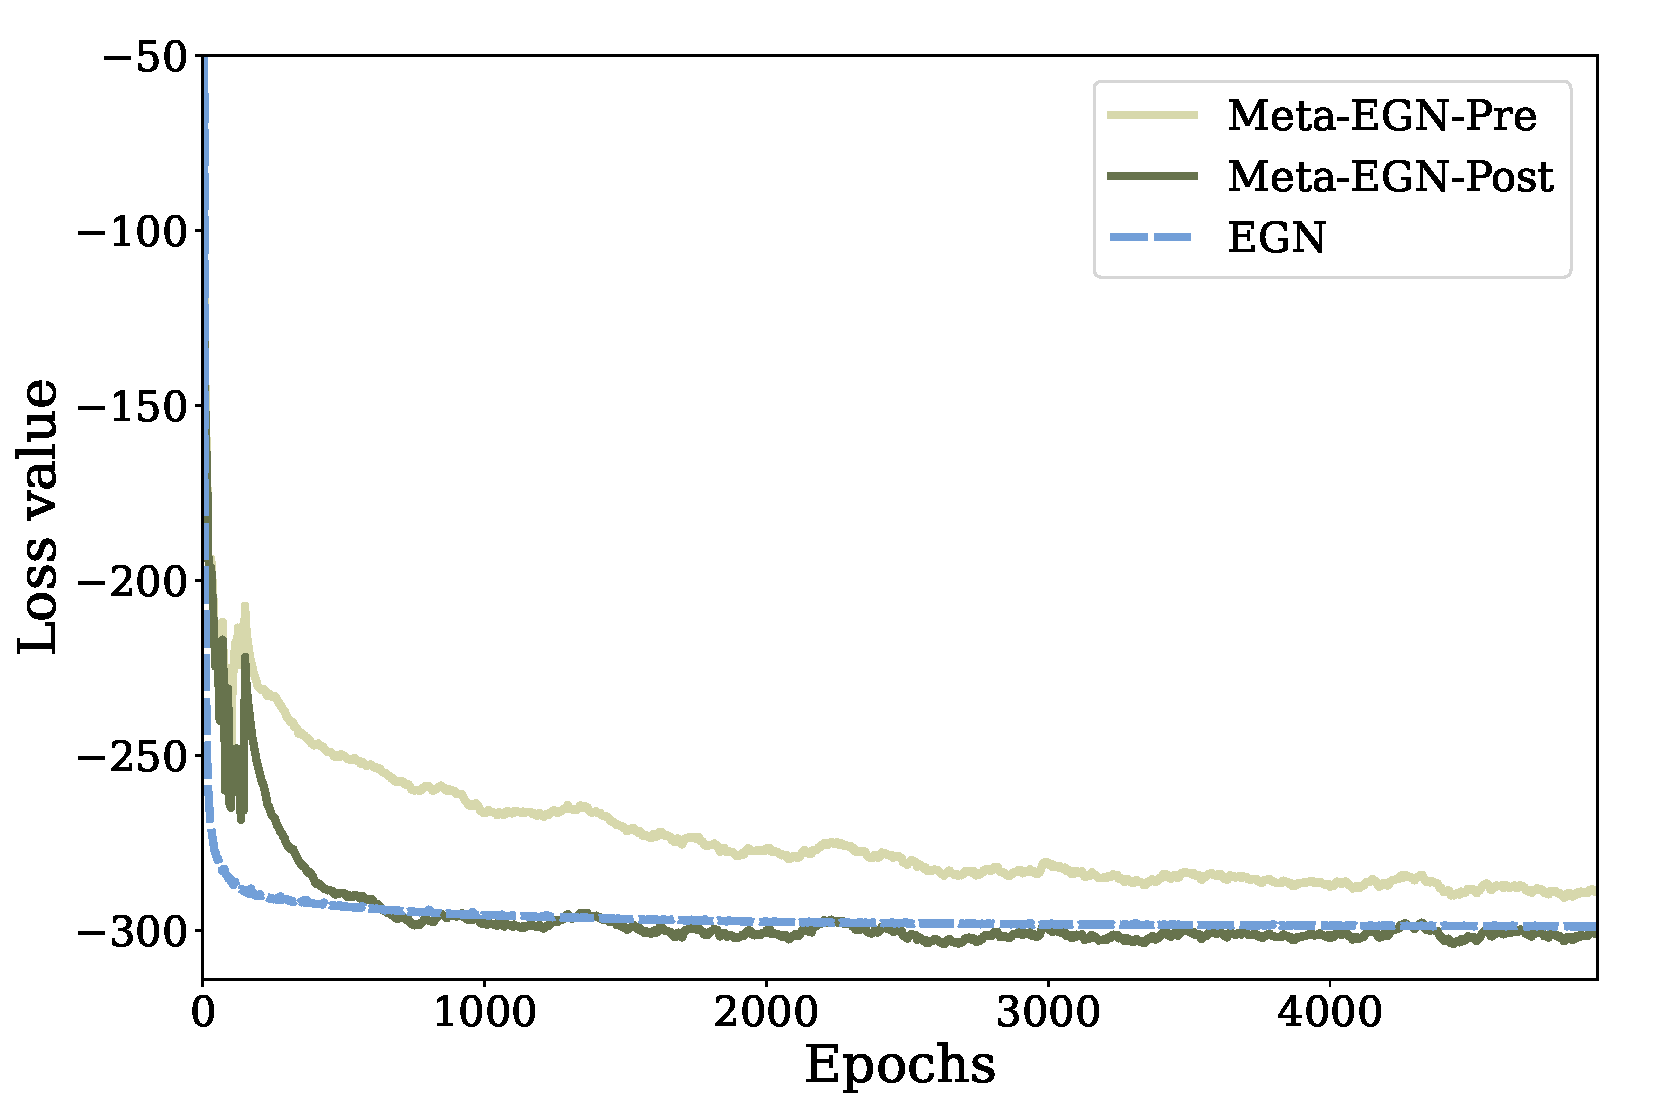
\includegraphics[width=\textwidth]{iclr2023/img/method/training_loss.pdf}
         \vspace{-0.6cm}
         \caption{Training Loss}
         \label{fig:dynamic_1}
     \end{subfigure}
     \hfill
     \begin{subfigure}[c]{0.32\textwidth}
         \centering
         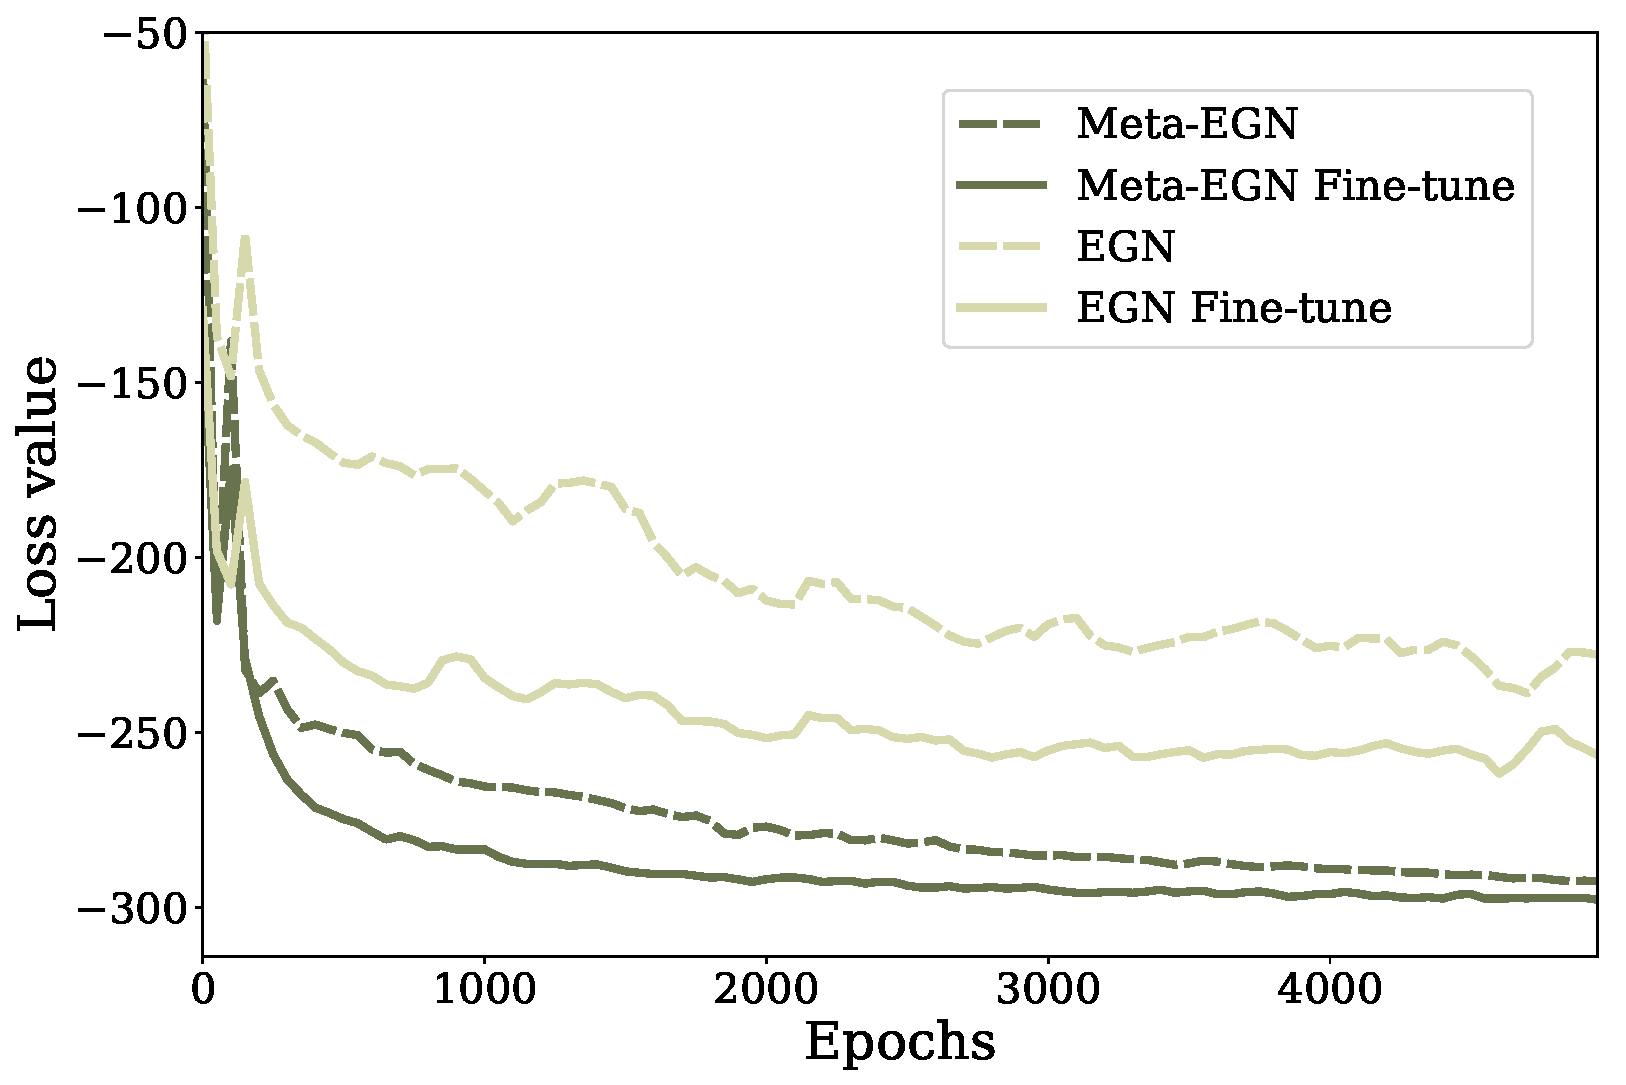
\includegraphics[width=\textwidth]{iclr2023/img/method/val_loss.pdf}
         \vspace{-0.6cm}
         \caption{Validation Loss}
         \label{method:fig_dynamic_2}
     \end{subfigure}
     \hfill
     \begin{subfigure}[c]{0.32\textwidth}
         \centering
         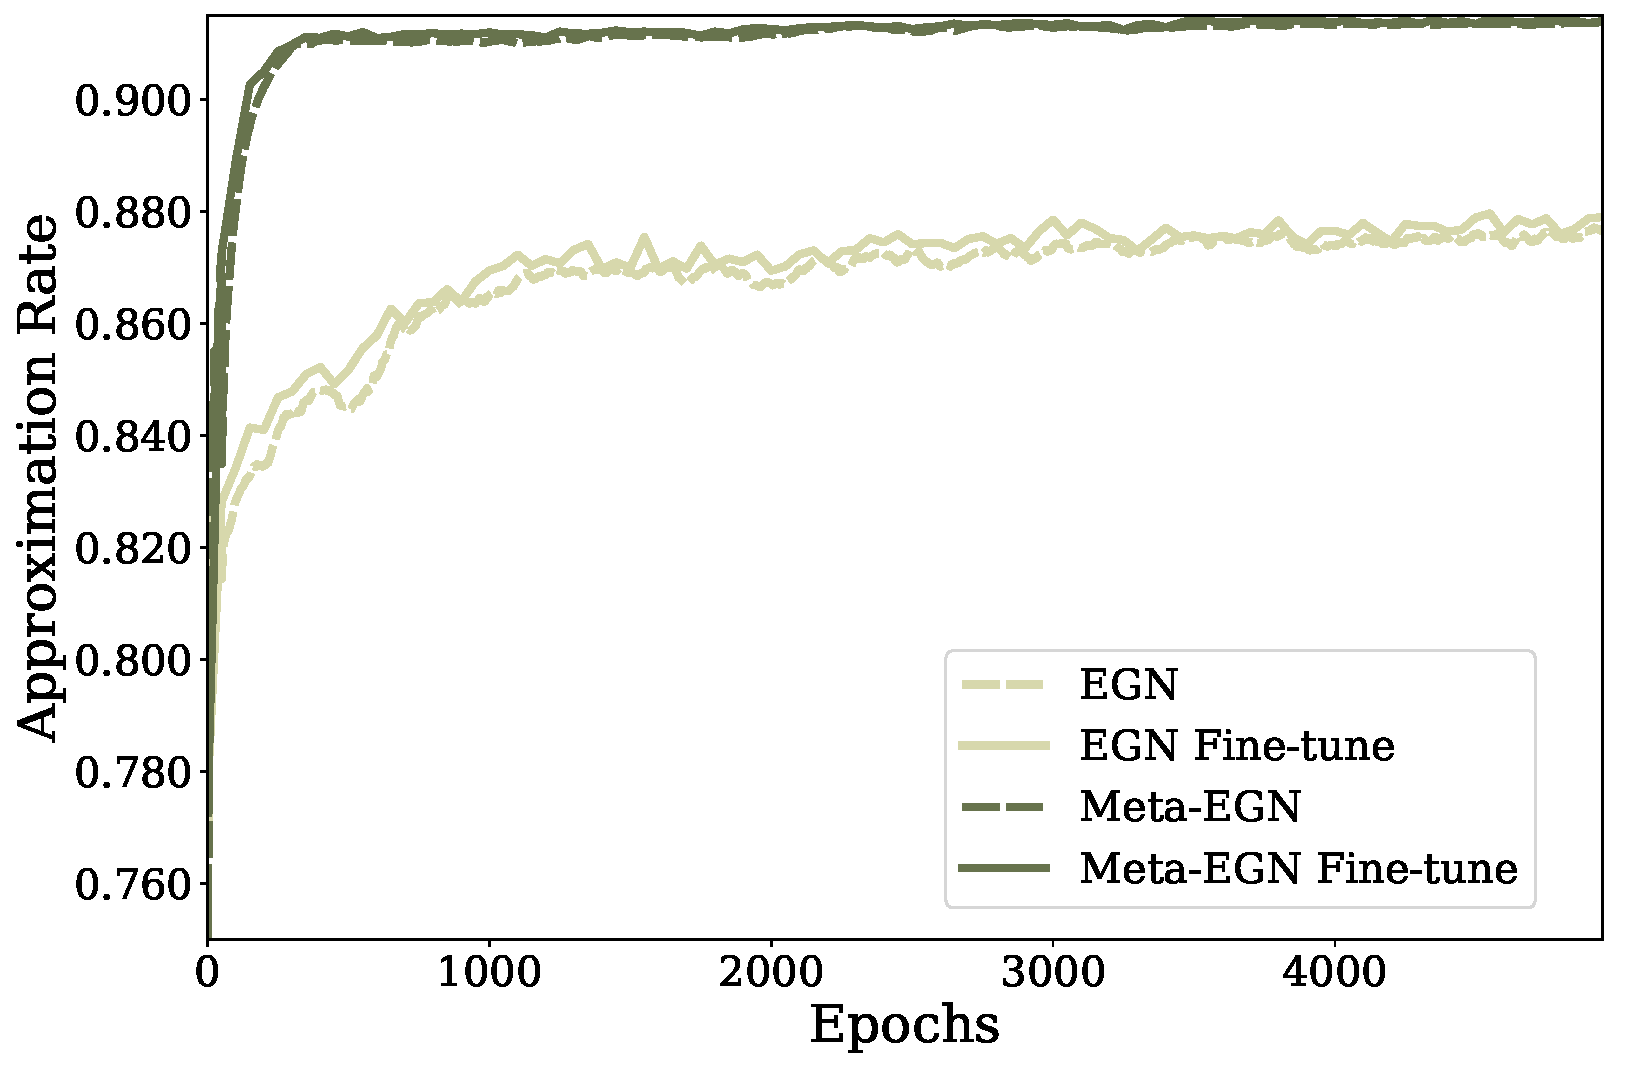
\includegraphics[width=\textwidth]{iclr2023/img/method/val_apr.pdf}
         \vspace{-0.6cm}
         \caption{Validation Approximation Rate }
         \label{fig:dynamic_3}
     \end{subfigure}
     \vspace{-0.2cm}
        \caption{Training/validating dynamics of \proj and EGN~\cite{karalias2020erdos} for the MIS problem.   Detailed experiment settings follow Sec.~\ref{sec:settings}.}
        \vspace{-0.2cm}%Other settings follow ~\citep{schuetz2022combinatorial,angelini2022cracking}.}  %In the training stage, the loss value of EGN framework is lower than that of \proj before the one-step inner gradient descent, but is higher than that of \proj after the one-step inner gradient descent. On validation set, a leap of the EGN losses of both before and after the fine-tuning could be observed, while the losses of \proj remain comparable to that during the training, revealing its higher generalization ability. Both the approximation rate (ApR) before and after fine-tuning of \proj on validation set outperforms EGN.}
        \label{fig:dynamic}
\end{figure}



We further simplify Eq.~\ref{eq:infinite_step} with some practical consideration. In fact, we may not allow further optimizing $\theta$ with so many gradient-descent steps for each instance, especially during the online test stage. As a proof of concept, we consider the case with only one-step gradient descent, which already gives good empirical results. Specifically, our training objective  follows
\begin{equation}
\label{eq:actual}
\begin{aligned}
\textbf{Our Objective:} \;\min_{\theta} \;\sum_{i=1}^m l_i(\theta), \quad \text{where}\; l_i(\theta) = l(\theta_i;G_i) \;\text{with $\theta_i=\theta -\alpha \nabla_\theta l(\theta;G_i)$.}
\end{aligned}
\end{equation}
Here, $\theta$ is to give a good initialization $\mathcal{A}_{\theta}(G_i)$ over each instance $G_i$ while $\theta_i$ is with one-step fine-tune to achieve a $G_i$-specified good solution $\mathcal{A}_{\theta_i}(G_i)$. 

Optimization in Eq.~\ref{eq:actual} can be implemented via the meta learning pipeline MAML~\citep{finn2017model}. We name the obtained model \proj and summarize its training and testing in Alg.~\ref{method:alg_table}. In step 3, \proj performs the one-step gradient descent on each training instance. Note that we consider two testing cases with or without fine-tuning because the latter saves much inference time. A simple extension of Theorem 1 in \citep{wang2022unsupervised} gives a performance guarantee for \proj in Theorem~\ref{thm:general_alpha} as follows. Here, for a test instance $G$, we even allow $l(\theta;G)$ to violate the original condition $l(\theta;G)<\beta$ in \citep{wang2022unsupervised} to some extent.  After one-step fine-tuning in step 9, the performance guarantee is still achievable. The detailed proof is in Appendix.~\ref{sec:proof-performance_guarantee}.% and the separated training/testing schedule is in Alg.~\ref{method:alg_table_train} and Alg.~\ref{method:alg_table_test} in the Appendix. %Interestingly, we observe that due to our training pipeline, \proj even without fine-tuning may 


\begin{theorem}[Performance Guarantee]
\label{thm:general_alpha}
Suppose the relaxations $f_r$ and $g_r$ are entry-wise concave as required in \citep{wang2022unsupervised}. Let $\theta$ denote the learned parameter after training.  Given a test instance $G$, suppose locally $l(\cdot;G)$ is $L$-smooth at $\theta$, i.e., $\|\nabla_{\theta'} l(\theta';G) - \nabla_{\theta} l(\theta;G)\|\leq L\|\theta' - \theta\|$ for all $\theta'$ that satisfies $\|\theta' - \theta\|\leq \epsilon$. Then, if \underline{$l(\theta;G) < \beta + \triangle$ (even if $l(\theta;G) \geq \beta$)}, for any $\alpha \in (0, 2/L)$ Meta-GNN with one-step finetuning outputs \underline{a feasible solution $X$ of good quality} $f(X;G)\leq l(\theta;G)-\triangle$. Here, $\triangle = \|\nabla_{\theta} l(\theta;G)\| \epsilon + \frac{1}{2L\alpha^2 - 4\alpha}\epsilon^2$ if $\epsilon < \alpha \|\nabla_{\theta} l(\theta;G)\|$ or $\triangle = (\alpha - \frac{L\alpha^2}{2})\|\nabla_{\theta}l(\theta;G)\|^2$ o.w..
\end{theorem}
%\begin{theorem}[Performance Guarantee]
%\label{thm:thm_performance_guarantee}
%Suppose the relaxations $f_r$ and $g_r$ are entry-wise concave as required in \citep{wang2022unsupervised}. Let $\theta$ denote the learned parameter after training.  Given a test instance $G$, suppose locally $l(\cdot;G)$ is $L$-smooth at $\theta$, i.e., $\|\nabla_{\theta'} l(\theta';G) - \nabla_{\theta} l(\theta;G)\|\leq L\|\theta' - \theta\|$ for all $\theta'$ that satisfies $\|\theta' - \theta\|\leq \epsilon$. Then, if \underline{$l(\theta;G) < \beta + \triangle$ (even if $l(\theta;G) \geq \beta$)}, there exists $\alpha$ such that Meta-GNN with one-step finetuning outputs \underline{a feasible solution $X$ of good quality} $f(X;G)\leq l(\theta;G)-\triangle$. Here, $\triangle = \|\nabla_{\theta} l(\theta;G)\|\epsilon - \frac{L}{2}\epsilon^2$ if $\epsilon< \frac{1}{L}\|\nabla_{\theta} l(\theta;G)\|$ or $\triangle=\frac{1}{2L}\|\nabla_{\theta} l(\theta;G)\|^2$ o.w..




% $<\beta$ 
% and $\theta_{G'}$ $\theta^*$ denote the corresponding local optimal parameter s.t. $\forall \theta \in \mathring{U}(\theta^*,\epsilon), l(\theta^*;G) < l(\theta;G)$, ($\mathring{U}(\cdot,\epsilon)$ is punctured neighborhood). Let $\beta > \max_{X \in \Omega} f(X;G)$ and $\min_{X\in \Omega}f(X;G)\geq 0$. Suppose the cost $f$ and constraint $g$ are entry-wise concave, $\theta$ achieves $l(\theta;G)<\beta$, and the inner fine-tune learning rate $\alpha \in (0,1/L_{\delta})$, where $L_{\delta}$ is the Lipschitz constant of the neighborhood $U(\theta;\delta)$ with a sufficiently small $\delta$,($\theta^*\notin U(\theta;\delta)$). Then with the fine-tuned parameter $\theta' = \theta - \alpha \nabla_{\theta} l(\theta;G)$, the relaxed solution $\bar{X} = \mathcal{A}_{\theta'}(G)$ generates a discrete solution $X \in \Omega$ such that $f(X;G) \leq l(\theta';G) \leq l(\theta;G)$ via the rounding process in Def.~\ref{def:rounding}.
%\vspace{-0.3cm}
%\end{theorem}



To better understand \proj, we show its training/testing dynamics in Fig.~\ref{fig:dynamic}. As we expected, the training loss of EGN is somewhere in-between the losses of \proj before and after the fine-tuning step. Training EGN is stabler and converges faster than training \proj. However, what is unexpected is that in validation, \proj has a much lower loss and achieves much better performance than EGN even before fine-tuning. 

This implies that \proj holds better generalization than EGN. We conjecture the reasons are as follows. First, the optimization landscape for CO problems is extremely non-convex~\citep{mezard2009information} due to the intersected feasible-infeasible regions and the high penalty coefficient $\beta$. 
EGN that has low losses for training instances may give a high loss even when the optimization landscape is just slightly shifted (from training to a test instance). However, the parameters of \proj are loosely tied to a local minimum for each training instance. Instead, those parameters, being aware of follow-up instance-wise fine-tuning steps, are likely to fall into some location close to a local minimum for each instance while being not trapped in any one of them, which makes the model robust to landscape shifts across instances. Second, a CO problem could vary a lot across graph instances even for those generated from the same distribution, especially when the instances are large. So, it is reasonable to view the problem over each instance as a separate but relevant task. %From this perspective, unsupervised learning for CO becomes a zero-shot learning task. 
Meta learning has shown good generalization when data distributions shift across tasks, which has empirical evidence in CV and NLP applications~\citep{jeong2020ood,conklin2021meta}.

%associates \proj with the capability of being adapted to the landscape shifts across instances. %See an illustration in Fig.~\ref{fig:landscape}.

As a summary, we provide a comparison between different unsupervised frameworks to solve CO problems in Table~\ref{tab:difference_methods}. Note that PI-GNN~\citep{schuetz2022combinatorial} is directly fine-tuned on each test instance without training so the fine-tuning time is long. Also, although PI-GNN also pursues instance-wise good solutions, its performance could be bad because it does not learn from training instances. The instance-wise solutions could be just bad local minima.  




% are easily trapped into valleys in the landscape with bad local minima. Having the per-instance gradient descent step during training, the model may understand better the lan 


% Slight perturbation on the parameters might substantially change the loss. 


% which leads to steep cliffs between the local minimum valleys, easily trapping the parameters in unsatisfactory ones. With the inner fine-tuning step, meta learning could potentially avoid the parameters from being trapped in bad local minima, leading to better performance and generalization.   


% in CO appears to be a more independent `task' rather than being as strongly connected with others as in common ML-based problems, which is similar with the `zero-shot learning' setting. Meta learning could naturally improve the out-of-distribution generalization~\citep{jeong2020ood,conklin2021meta} in few-shot learning tasks. 2) The optimization landscape of unsupervised learning for CO is much more intricate with high variance~\citep{mezard2009information} due to the scattered feasible-infeasible regions and the high penalty coefficient $\beta$. Any slight disturbance on the parameters might subvert the loss function, which leads to steep cliffs between the local minimum valleys, easily trapping the parameters in unsatisfactory ones. With the inner fine-tuning step, meta learning could potentially avoid the parameters from being trapped in bad local minima, leading to better performance and generalization. 3) During the training procedure, meta learning aims to guarantee the performance in the linear local regime before and after the inner fine-tune step, thus tending to choose the initialization inside deeper and better valleys, which results in better performance of the Mega-EGN over EGN even without the fine-tune step. Comparison between \proj with the other unsupervised methods is discussed in Tab.~\ref{method:tab_difference_methods}.


% However, what is 

% \proj boosts the performance of the previous framework EGN, as illustrated in the training dynamics of the max independent set problem on random-regular graphs in Fig.~\ref{method:fig_dynamic}. According to the training dynamics, the training loss of EGN is between those of \proj before and after its inner fine-tune step. Both the validation losses of EGN before and after fine-tune are much higher than those of \proj. Also, the validation approximation rate of \proj even with the learnt initialization still largely outperforms that of EGN either before or after the fine-tune. We attribute these observations to meta learning's ability in improving not only the performance but also the generalization ability. The reason behind such improvement could be summarized as follows: 1) Each instance in CO appears to be a more independent `task' rather than being as strongly connected with others as in common ML-based problems, which is similar with the `zero-shot learning' setting. Meta learning could naturally improve the out-of-distribution generalization~\citep{jeong2020ood,conklin2021meta} in few-shot learning tasks. 2) The optimization landscape of unsupervised learning for CO is much more intricate with high variance~\citep{mezard2009information} due to the scattered feasible-infeasible regions and the high penalty coefficient $\beta$. Any slight disturbance on the parameters might subvert the loss function, which leads to steep cliffs between the local minimum valleys, easily trapping the parameters in unsatisfactory ones. With the inner fine-tuning step, meta learning could potentially avoid the parameters from being trapped in bad local minima, leading to better performance and generalization. 3) During the training procedure, meta learning aims to guarantee the performance in the linear local regime before and after the inner fine-tune step, thus tending to choose the initialization inside deeper and better valleys, which results in better performance of the Mega-EGN over EGN even without the fine-tune step. Comparison between \proj with the other unsupervised methods is discussed in Tab.~\ref{method:tab_difference_methods}. 



%itself by regarding each training instance as an independent task as well as a pseudo-new task. Then whenever an unseen testing instance $G'$ is encountered, if some time for fine-tuning is allowed, one-step or even multiple steps (depending on the time limitation) fine-tuning is conducted on the testing instance to obtain the instance-particular parameter $\theta_{G'}$, aiming to move the initialization $\theta$ closer towards the per-instance optimality. $\theta_{G'}$ is then utilized to obtain $\bar{X} = \mathcal{A}_{\theta_{G'}}(G')$, followed by the rounding procedure in Def.~\ref{method:def_rounding} with performance guarantee (shown in Thm.~\ref{method:thm_performance_guarantee} below) to obtain the discrete solution $X$. If extreme rapid inference time is required, the initialization $\theta$ could be directly used to obtain the relaxed $\bar{X}$ and continue the same rounding. Note that although many of the traditional tasks (i.e. classification or regression) are also optimized for the optimality in the expectation sense, these tasks could not do anything better towards the optimality for single instances, because it is the unsupervised learning framework that gets rid of the labels and enables our one-step fine-tune on unseen testing instances to pursue optimality for a single instance. 




% Although this is not ideal, we expect that if test instances follow the same/similar distribution of training instances 

% draw on the heuristics from historical graphs to obtain a good initialization $\theta$ such that a limited step (one-step in our case considering time efficiency) fine-tuning of $\theta$ on the testing instance could further help the model leap closer to the per-instance optimality. The idea naturally aligns with the concept of meta learning, our loss function is thus defined as follows:
% \begin{equation}
% \label{method:meta_loss}
% \begin{aligned}
% \tilde{l}(\theta,G): \triangleq f(\bar{X};G)+\beta g(\bar{X};G), \quad \bar{X} = \mathcal{A}_{\theta_G}(G) \quad \text{s.t.} \quad \theta_G = \theta - \nabla_\theta l(\theta, G),
% \end{aligned}
% \end{equation}Our optimization objective could be summarized as:
% \begin{equation}
% \label{method:meta_goal}
% \begin{aligned}
% \min_{\theta} \mathbb{E}_{d \sim \mathbb{P}_G} \tilde{l}(\theta,G).
% \end{aligned}
% \end{equation}



% To narrow the gap above, our idea is to draw on the heuristics from historical graphs to obtain a good initialization $\theta$ such that a limited step (one-step in our case considering time efficiency) fine-tuning of $\theta$ on the testing instance could further help the model leap closer to the per-instance optimality. The idea naturally aligns with the concept of meta learning, our loss function is thus defined as follows:
% \begin{equation}
% \label{method:meta_loss}
% \begin{aligned}
% \tilde{l}(\theta,G): \triangleq f(\bar{X};G)+\beta g(\bar{X};G), \quad \bar{X} = \mathcal{A}_{\theta_G}(G) \quad \text{s.t.} \quad \theta_G = \theta - \nabla_\theta l(\theta, G),
% \end{aligned}
% \end{equation}Our optimization objective could be summarized as:
% \begin{equation}
% \label{method:meta_goal}
% \begin{aligned}
% \min_{\theta} \mathbb{E}_{d \sim \mathbb{P}_G} \tilde{l}(\theta,G).
% \end{aligned}
% \end{equation}

% With the training objective above, we train the unsupervised learning framework following the procedure as illustrated in Alg.~\ref{method:alg_table}: \proj performs meta learning with one step inner gradient descent on each training instance itself by regarding each training instance as an independent task as well as a pseudo-new task. Then whenever an unseen testing instance $G'$ is encountered, if some time for fine-tuning is allowed, one-step or even multiple steps (depending on the time limitation) fine-tuning is conducted on the testing instance to obtain the instance-particular parameter $\theta_{G'}$, aiming to move the initialization $\theta$ closer towards the per-instance optimality. $\theta_{G'}$ is then utilized to obtain $\bar{X} = \mathcal{A}_{\theta_{G'}}(G')$, followed by the rounding procedure in Def.~\ref{method:def_rounding} with performance guarantee (shown in Thm.~\ref{method:thm_performance_guarantee} below) to obtain the discrete solution $X$. If extreme rapid inference time is required, the initialization $\theta$ could be directly used to obtain the relaxed $\bar{X}$ and continue the same rounding. Note that although many of the traditional tasks (i.e. classification or regression) are also optimized for the optimality in the expectation sense, these tasks could not do anything better towards the optimality for single instances, because it is the unsupervised learning framework that gets rid of the labels and enables our one-step fine-tune on unseen testing instances to pursue optimality for a single instance. 



% \begin{theorem}[\proj's Performance Guarantee]
% \label{method:thm_performance_guarantee}
% Let $\theta$ denote the learnt initialization from training data, $\theta^*$ denote the corresponding local optimal parameter s.t. $\forall \theta \in \mathring{U}(\theta^*,\epsilon), l(\theta^*;G) < l(\theta;G)$, ($\mathring{U}(\cdot,\epsilon)$ is punctured neighborhood). Let $\beta > \max_{X \in \Omega} f(X;G)$ and $\min_{X\in \Omega}f(X;G)\geq 0$. Suppose the cost $f$ and constraint $g$ are entry-wise concave, $\theta$ achieves $l(\theta;G)<\beta$, and the inner fine-tune learning rate $\\alpha \in (0,1/L_{\delta})$, where $L_{\delta}$ is the Lipschitz constant of the neighborhood $U(\theta;\delta)$ with a sufficiently small $\delta$,($\theta^*\notin U(\theta;\delta)$). Then with the fine-tuned parameter $\theta' = \theta - \\alpha \nabla_{\theta} l(\theta;G)$, the relaxed solution $\bar{X} = \mathcal{A}_{\theta'}(G)$ generates a discrete solution $X \in \Omega$ such that $f(X;G) \leq l(\theta';G) \leq l(\theta;G)$ via the rounding process in Def.~\ref{def:rounding}.
% \vspace{-0.3cm}
% \end{theorem}

% \begin{algorithm}[h]
% \caption{\proj for CO}
% \label{method:alg_table}
% \begin{algorithmic}[1]
% \Require $\mathbb{P}_G$: distribution over the CO instances
% \Require $\alpha, \\alpha$: step size hyper-parameters
% \State randomly initialize $\theta$
% \While{not done} \Comment{Training starts}
% \State Sample instances $G_i \sim \mathbb{P}_G$ 
% %\For {$K$ steps}
% \ForAll{$G_i$}
% \State Evaluate $\nabla_{\theta}l(\theta;G_i)$
% \State Compute adapted parameters with gradient descent: $\theta' = \theta - \alpha \nabla_{\theta}l(\theta;G_i)$
% \EndFor
% \State Update: $\theta \gets \theta - \\alpha \nabla_{\theta} \sum_{G_i \sim \mathbb{P}_G} l(\theta';G_i)$
% %\EndFor
% \EndWhile \Comment{Training ends}
% \State For any given testing instance $G'$: \Comment{Testing starts}
% \If {fine-tune time is allowed}
% \State Fine-tune the parameters: $\theta_{G'} \gets \theta - \\alpha \nabla_{\theta} l(\theta; G')$ \Comment {Fine-tune for per-instance optimality}
% \State Inference the relaxed solution with fine-tuned parameters: $\bar{X} = \mathcal{A}_{\theta_{G'}} (\theta_{G'};G')$
% \State Rounding for discrete solution
% \Else
% \State Inference the relaxed solution directly: $\bar{X} = \mathcal{A}_{\theta} (\theta;G')$
% \State Rounding for discrete solution
% \EndIf \Comment{Testing ends}
% \end{algorithmic}
% \end{algorithm}

% \begin{figure}[t]
%      \centering
%      \begin{subfigure}[c]{0.32\textwidth}
%          \centering
%          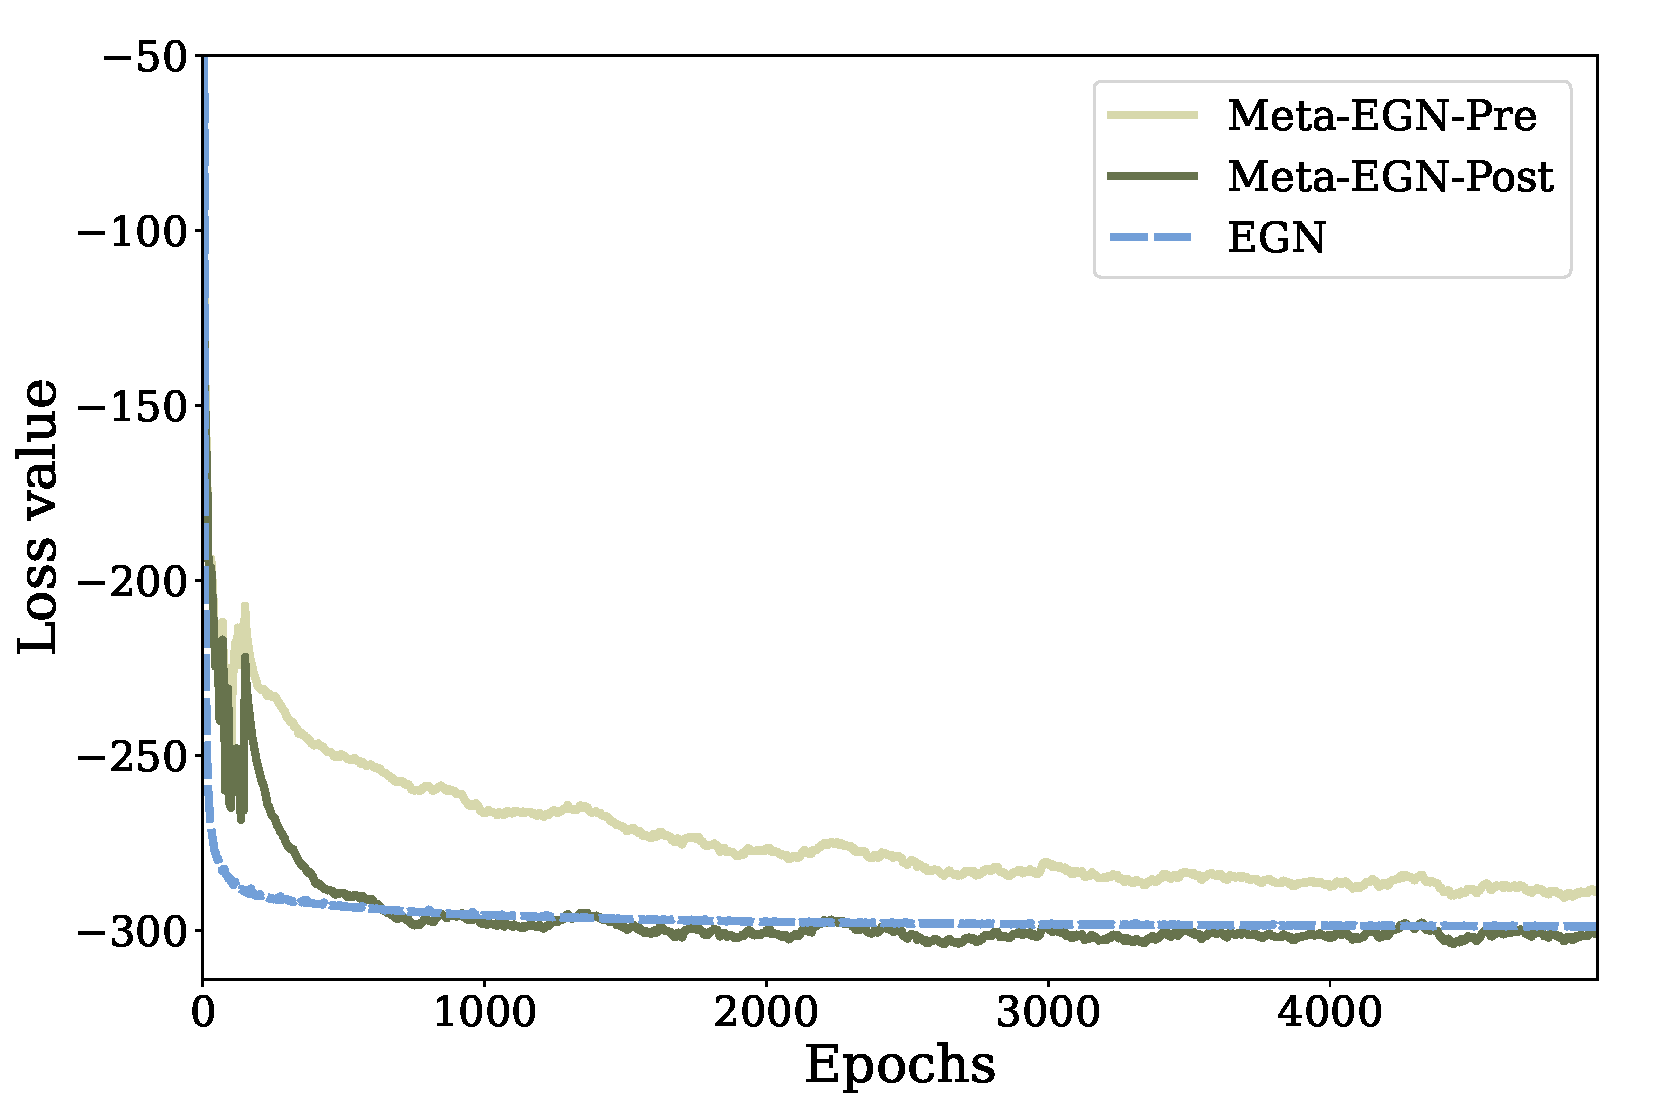
\includegraphics[width=\textwidth]{iclr2023/img/method/training_loss.pdf}
%          \vspace{-0.6cm}
%          \caption{Training Loss}
%          \label{method:fig_dynamic_1}
%      \end{subfigure}
%      \hfill
%      \begin{subfigure}[c]{0.32\textwidth}
%          \centering
%          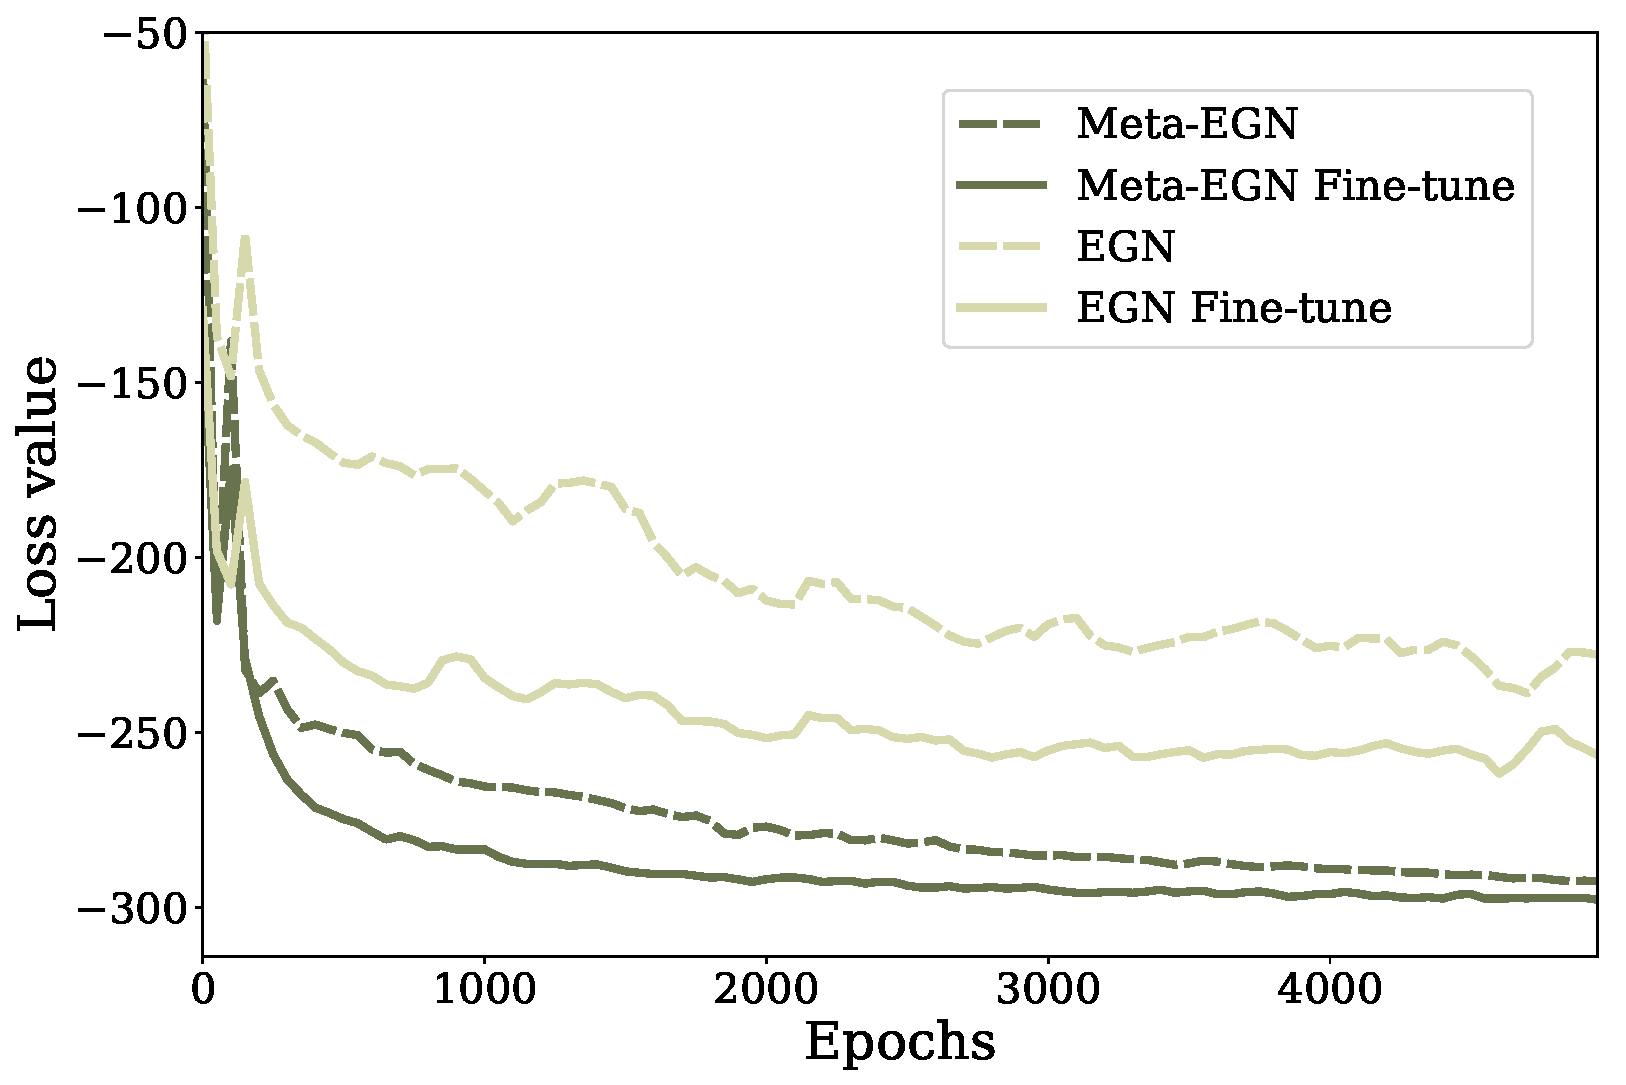
\includegraphics[width=\textwidth]{iclr2023/img/method/val_loss.pdf}
%          \vspace{-0.6cm}
%          \caption{Validation Loss}
%          \label{method:fig_dynamic_2}
%      \end{subfigure}
%      \hfill
%      \begin{subfigure}[c]{0.32\textwidth}
%          \centering
%          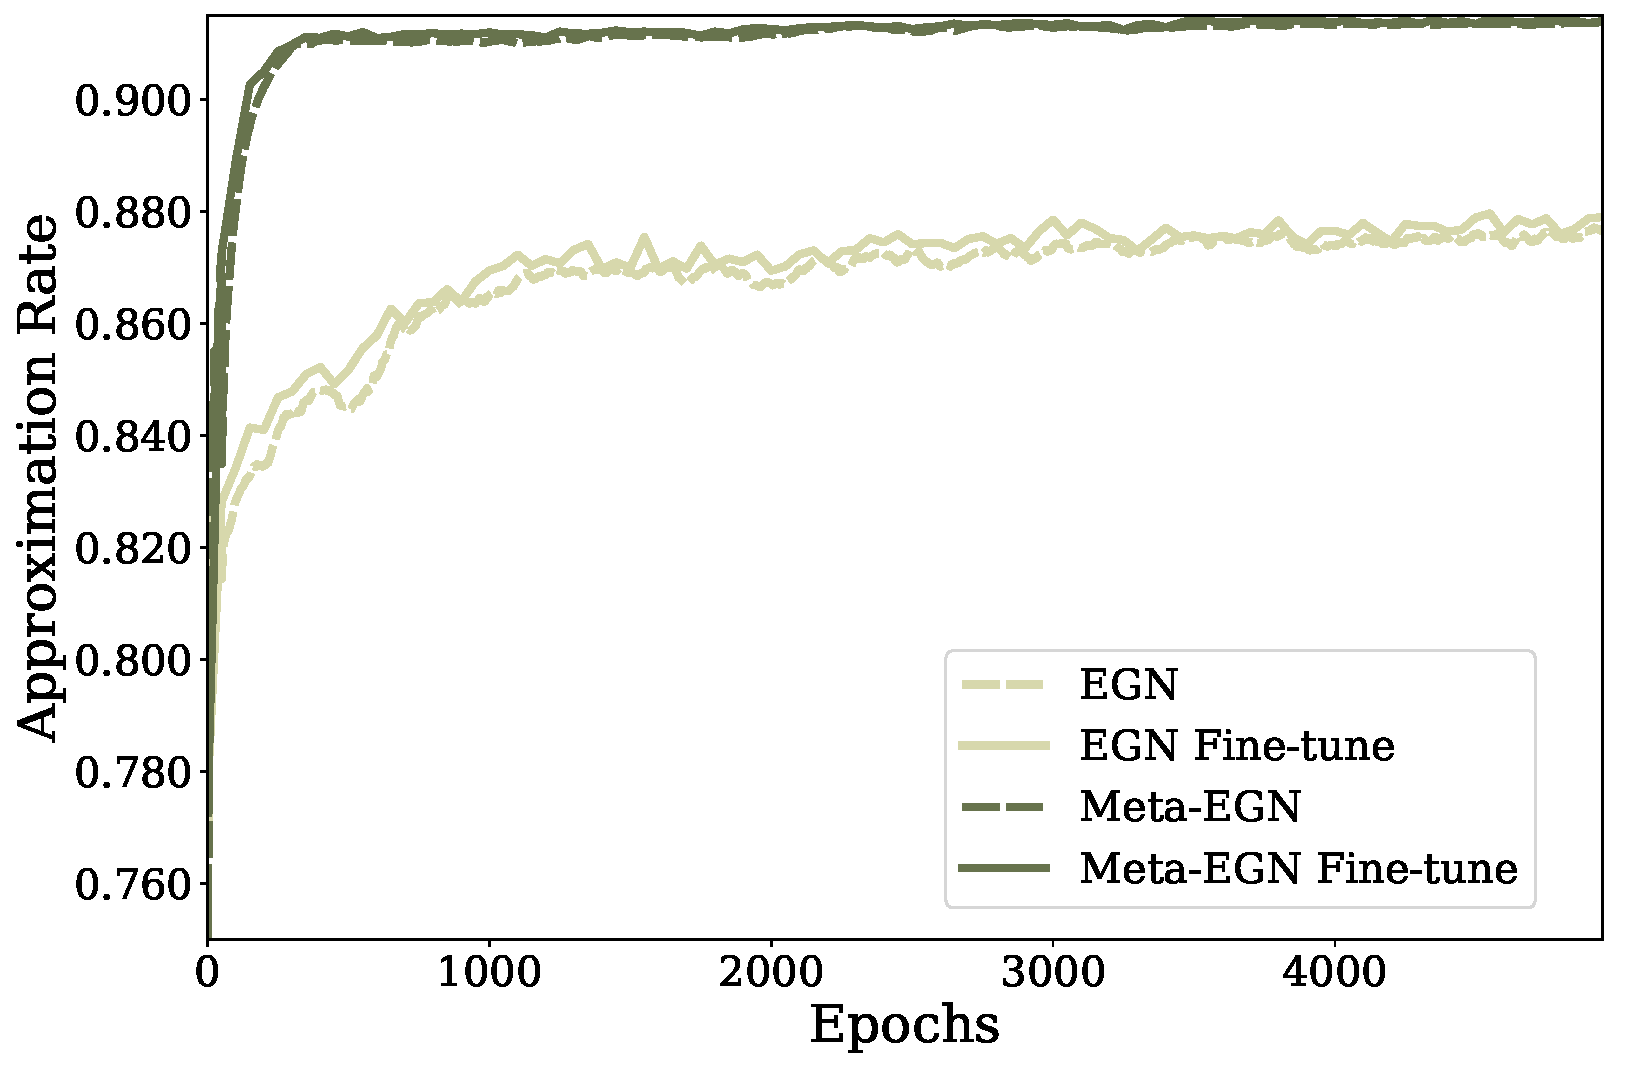
\includegraphics[width=\textwidth]{iclr2023/img/method/val_apr.pdf}
%          \vspace{-0.6cm}
%          \caption{Validation Approximation Rate}
%          \label{method:fig_dynamic_3}
%      \end{subfigure}
%      \vspace{-0.3cm}
%         \caption{Training dynamics of max independent set problem with mixed degrees $(3,5,7,10,20)$ on random-regular graphs with $1000$ vertices, where the settings follow ~\cite{schuetz2022combinatorial,angelini2022cracking}. In the training stage, the loss value of EGN framework is lower than that of \proj before the one-step inner gradient descent, but is higher than that of \proj after the one-step inner gradient descent. On validation set, a leap of the EGN losses of both before and after the fine-tuning could be observed, while the losses of \proj remain comparable to that during the training, revealing its higher generalization ability. Both the approximation rate (ApR) before and after fine-tuning of \proj on validation set outperforms EGN.}
%         \label{method:fig_dynamic}
% \end{figure}

% \proj boosts the performance of the previous framework EGN, as illustrated in the training dynamics of the max independent set problem on random-regular graphs in Fig.~\ref{method:fig_dynamic}. According to the training dynamics, the training loss of EGN is between those of \proj before and after its inner fine-tune step. Both the validation losses of EGN before and after fine-tune are much higher than those of \proj. Also, the validation approximation rate of \proj even with the learnt initialization still largely outperforms that of EGN either before or after the fine-tune. We attribute these observations to meta learning's ability in improving not only the performance but also the generalization ability. The reason behind such improvement could be summarized as follows: 1) Each instance in CO appears to be a more independent `task' rather than being as strongly connected with others as in common ML-based problems, which is similar with the `zero-shot learning' setting. Meta learning could naturally improve the out-of-distribution generalization~\citep{jeong2020ood,conklin2021meta} in few-shot learning tasks. 2) The optimization landscape of unsupervised learning for CO is much more intricate with high variance~\citep{mezard2009information} due to the scattered feasible-infeasible regions and the high penalty coefficient $\beta$. Any slight disturbance on the parameters might subvert the loss function, which leads to steep cliffs between the local minimum valleys, easily trapping the parameters in unsatisfactory ones. With the inner fine-tuning step, meta learning could potentially avoid the parameters from being trapped in bad local minima, leading to better performance and generalization. 3) During the training procedure, meta learning aims to guarantee the performance in the linear local regime before and after the inner fine-tune step, thus tending to choose the initialization inside deeper and better valleys, which results in better performance of the Mega-EGN over EGN even without the fine-tune step. Comparison between \proj with the other unsupervised methods is discussed in Tab.~\ref{method:tab_difference_methods}. 

% \begin{table}[h]
% \setlength\tabcolsep{1pt}
% \centering
% \footnotesize
% \begin{tabular}{@{}ccccc@{}}
% \toprule
%  &
%   \begin{tabular}[c]{@{}c@{}}EGN\\ ~\citep{karalias2020erdos}\end{tabular} &\begin{tabular}[c]{@{}c@{}}P-I GNN\\ ~\citep{schuetz2022combinatorial}\end{tabular}
%   &
%   \begin{tabular}[c]{@{}c@{}}\proj\\ (Ours)\end{tabular} &
%   \begin{tabular}[c]{@{}c@{}}Classical Solver\\ ~\cite{Gurobi} \end{tabular} \\ \midrule
% Goal           &     $\mathbb{E}_{D\sim \mathbb{P}_D} l(\theta;D)$     &   $l(\theta;D)$   &    $\mathbb{E}_{D\sim \mathbb{P}_D} \tilde{l}(\theta;D)$    &   $f(X;D) \  \text{s.t.} \  X \in \Omega$   \\
% Training  & Yes        &   No   & Yes & No   \\
% Fine-tune time & No & Very long   & Short  & Long \\
% Generalization &  Good        & - & Better & -    \\ \bottomrule
% \end{tabular}
% \caption{Comparison between our framework and the previous unsupervised frameworks.}
% \label{method:tab_difference_methods}
% \end{table}

\begin{table}[t]
\setlength\tabcolsep{1pt}
\centering
%\footnotesize
\caption{Comparison between different unsupervised frameworks. $G$ denotes the test instance and $G_i$, $1\leq i\leq m$ are training instances. The standard EGN pipeline does not adopt any fine-tuning.}
\label{tab:difference_methods}
\vspace{-3mm}
\resizebox{1\textwidth}{!}{
\begin{tabular}{@{}ccccc@{}}
\toprule
 &
  \begin{tabular}[c]{@{}c@{}}EGN\\ ~\citep{karalias2020erdos}\end{tabular} &\begin{tabular}[c]{@{}c@{}}P-I GNN\\ ~\citep{schuetz2022combinatorial}\end{tabular}
   &
  \begin{tabular}[c]{@{}c@{}}\proj\\ (Ours)\end{tabular} &
  \begin{tabular}[c]{@{}c@{}}Classical Solver\\ ~\cite{Gurobi} \end{tabular} \\ \midrule
Obj. to optimize the NN           &     $\sum_{i=1}^m l(\theta;G_i)$     &   $l(\theta;G)$   &    $\sum_{i=1}^m l(\theta -\nabla_{\theta} l(\theta;G_i) ;G_i)$    &   $f(X;G) \  \text{s.t.} \  X \in \Omega$   \\
Training or not  & Yes        &   No   & Yes & No   \\
Fine-tune timing & No & Long   & Short/No  &  Long  \\
Generalization &  Good        & - & Better & -    \\ \bottomrule
\end{tabular}}
\vspace{-1mm}
\end{table}